\section{What is a Mixture of Experts (MoE)?}
\begin{frame}[allowframebreaks]{}
    \LARGE What is a Mixture of Experts (MoE)?
\framebreak
    \begin{figure}[h]
        \centering
        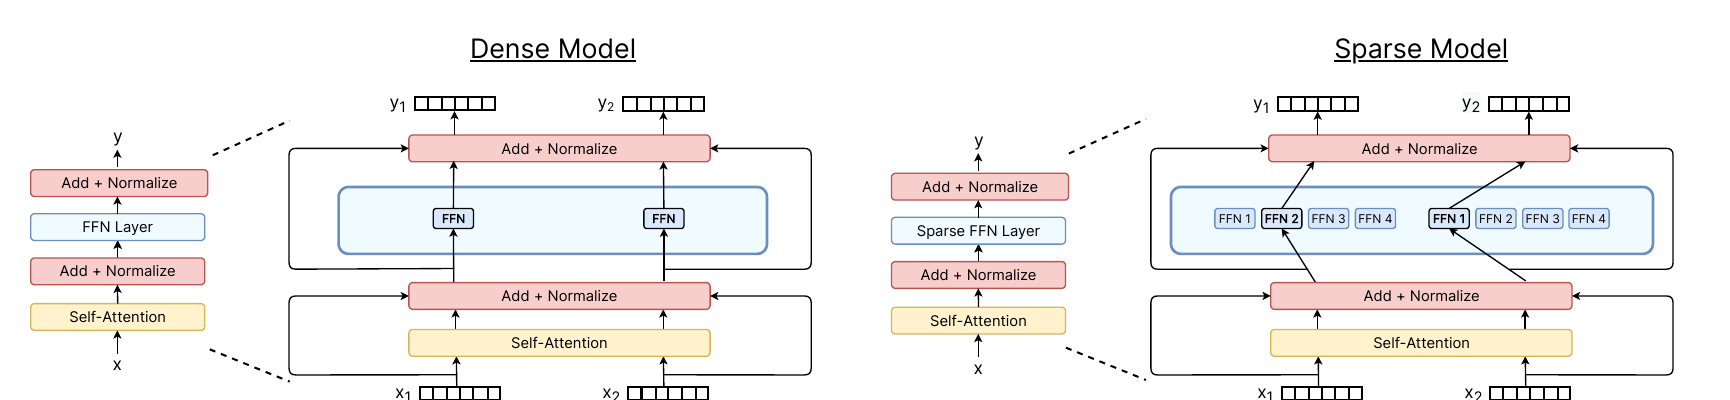
\includegraphics[width=\textwidth,height=0.9\textheight,keepaspectratio]{images/lrm+moe/dense_vs_sparse_transformer_fedus_fig1.png}
        \caption*{\scriptsize A dense model sends every token through the same FFN; a sparse expert model routes each token to a subset of the expert FFNs. Source: \href{https://arxiv.org/abs/2209.01667}{Fedus, Dean \& Zoph (2022)}, Fig.~1.}
    \end{figure}
\end{frame}

\begin{frame}[allowframebreaks]{What is a Mixture of Experts (MoE)?}
    \begin{itemize}
        \item \textbf{Definition}
        \begin{itemize}
            \item It combines multiple specialized models, called experts.
            \item Each expert focuses on a specific subset of data or task.
            \item This specialization enables efficient and effective learning.
        \end{itemize}
        \item \textbf{How does it work?}
        \begin{itemize}
            \item MoE uses a gating mechanism.
            \item The gate selects which expert(s) to use for a given input.
            \item The model adapts its behavior dynamically based on the input.
            \item It draws on the strengths of different experts.
        \end{itemize}
    \end{itemize}

    \framebreak

    \begin{itemize}
        \item \textbf{Why is it important?}
        \begin{itemize}
            \item MoE models handle large-scale problems efficiently.
            \item They distribute workload across multiple experts.
            \item Combining expertise of different models improves performance on complex tasks.
        \end{itemize}
        \item \textbf{Challenges}
        \begin{itemize}
            \item Training MoE models is computationally expensive.
            \item Multiple experts need to be trained.
            \item Designing effective gating mechanisms is difficult.
            \item Ensuring balanced expert utilization is challenging.
        \end{itemize}
    \end{itemize}

    \framebreak

    \textbf{Examples of Mixture of Experts Models}
    \begin{itemize}
        \item \textbf{Switch Transformer}
        \begin{itemize}
            \item Uses a gating mechanism to select one or a few experts per input.
            \item Activates only a small subset of experts at a time.
            \item Enables large-scale models without excessive computational costs.
            \item \textit{Example:}
            \begin{itemize}
                \item Handles language modeling and translation.
                \item Uses specialized experts for different aspects of the task.
            \end{itemize}
        \end{itemize}
    \framebreak
        \begin{figure}[h]
            \centering
            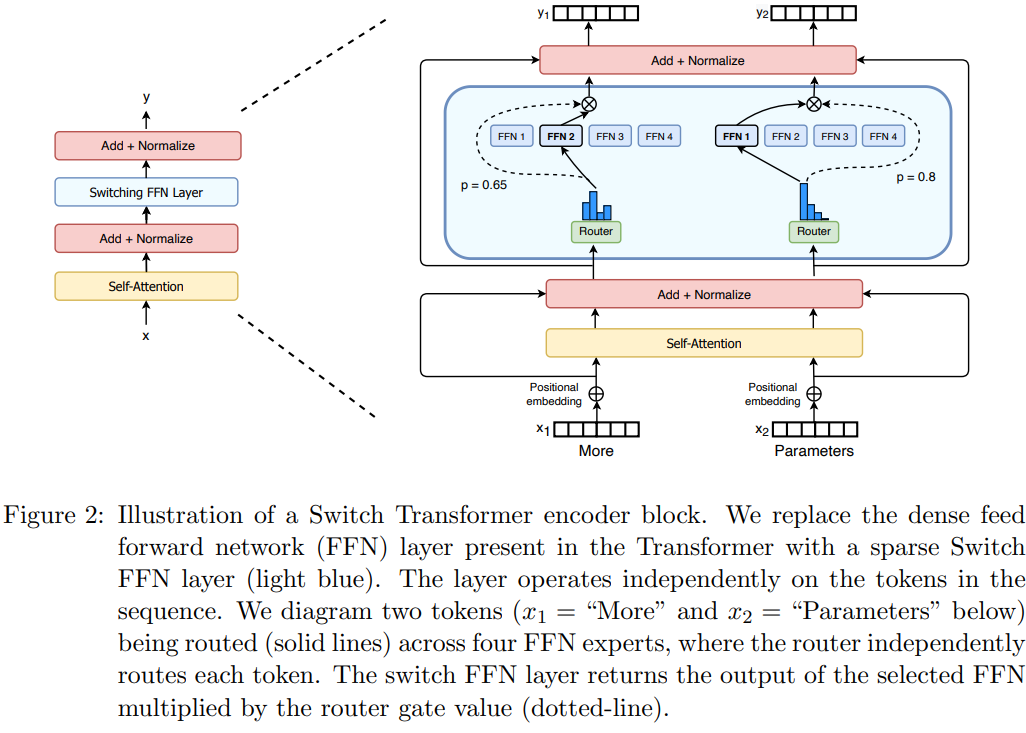
\includegraphics[width=\linewidth,height=0.84\textheight,keepaspectratio]{images/lrm+moe/switch-transformer.png}

            {\usebeamerfont{caption}\usebeamercolor[fg]{caption}Source: \href{https://arxiv.org/pdf/2101.03961}{Fedus et al. (2021)}}
        \end{figure}
    \framebreak
        \item \textbf{GShard}
        \begin{itemize}
            \item Scales up the number of experts for very large datasets and models.
            \item Distributes computation across multiple devices.
            \item Enables efficient training of large models.
            \item \textit{Example:}
            \begin{itemize}
                \item Trained a 600B-parameter MoE Transformer for machine translation from 100 languages into English.
                \item Utilizes many experts to process different data parts.
            \end{itemize}
        \end{itemize}
    \framebreak
        \begin{figure}[h]
            \centering
            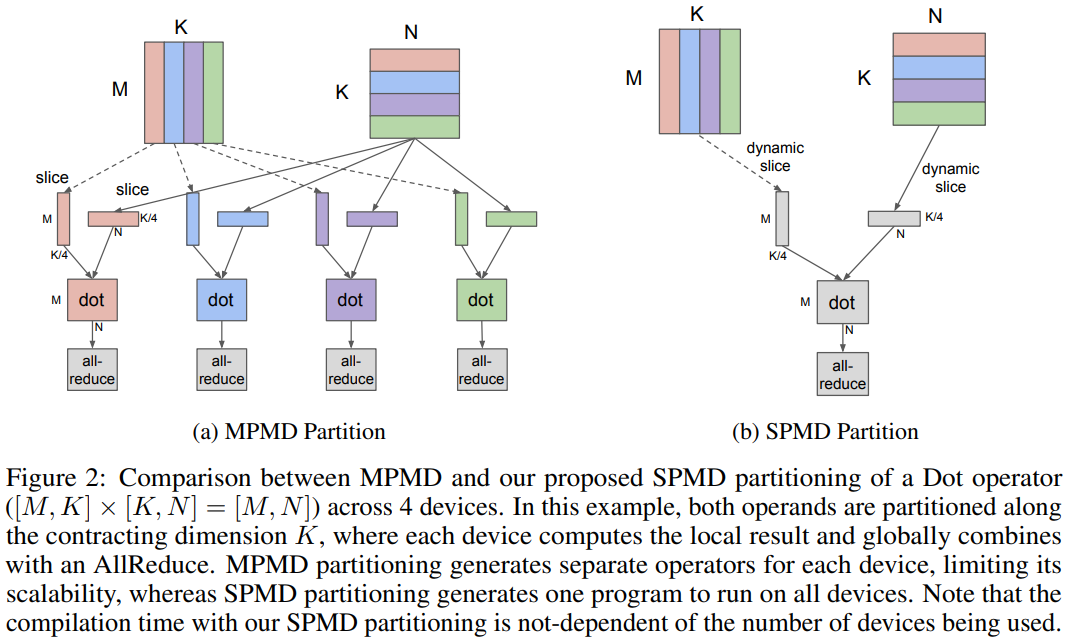
\includegraphics[width=\linewidth,height=0.8\textheight,keepaspectratio]{images/lrm+moe/gshard-compare.png}

            {\usebeamerfont{caption}\usebeamercolor[fg]{caption}\scriptsize GShard's SPMD (single program, multiple data) partitioner splits a single operator across devices, so compilation cost stays independent of how many devices are used. Source: \href{https://arxiv.org/pdf/2006.16668}{Lepikhin et al. (2020)}, Fig.~2.}
        \end{figure}
    \framebreak
        \item \textbf{MoE in BERT}
        \begin{itemize}
            \item BERT can be extended with MoE layers.
            \item MoE layers enhance performance on specific tasks.
            \item Allows BERT to dynamically select experts based on input.
            \item Improves ability to handle diverse tasks.
            \item \textit{Example:}
            \begin{itemize}
                \item MoE-enhanced BERT performs better on sentiment analysis and question answering.
                \item Uses specialized experts for different input types.
            \end{itemize}
        \end{itemize}
        \item \textbf{MicroBERT: Distilling MoE-Based Knowledge}
        \begin{itemize}
            \item Distills a full-size BERT teacher into a much smaller student.
            \item The distillation signal is a sentence-level feature alignment loss guided by a Mixture-of-Experts layer.
            \item A discriminator trained adversarially pushes the student's predictions towards the teacher's.
            \item Targets resource-constrained environments.
            \item \textit{Key Points:}
            \begin{itemize}
                \item Teacher: BERT; Student: MicroBERT. The MoE sits in the distillation path, not in the teacher backbone.
                \item Reported to perform about 2.24\% better than TinyBERT on GLUE at a reduced model size.
                \item Reduces inference time and memory usage.
                \item Suitable for deployment on edge devices.
            \end{itemize}
        \end{itemize}
    \framebreak
        \begin{figure}[h]
            \centering
            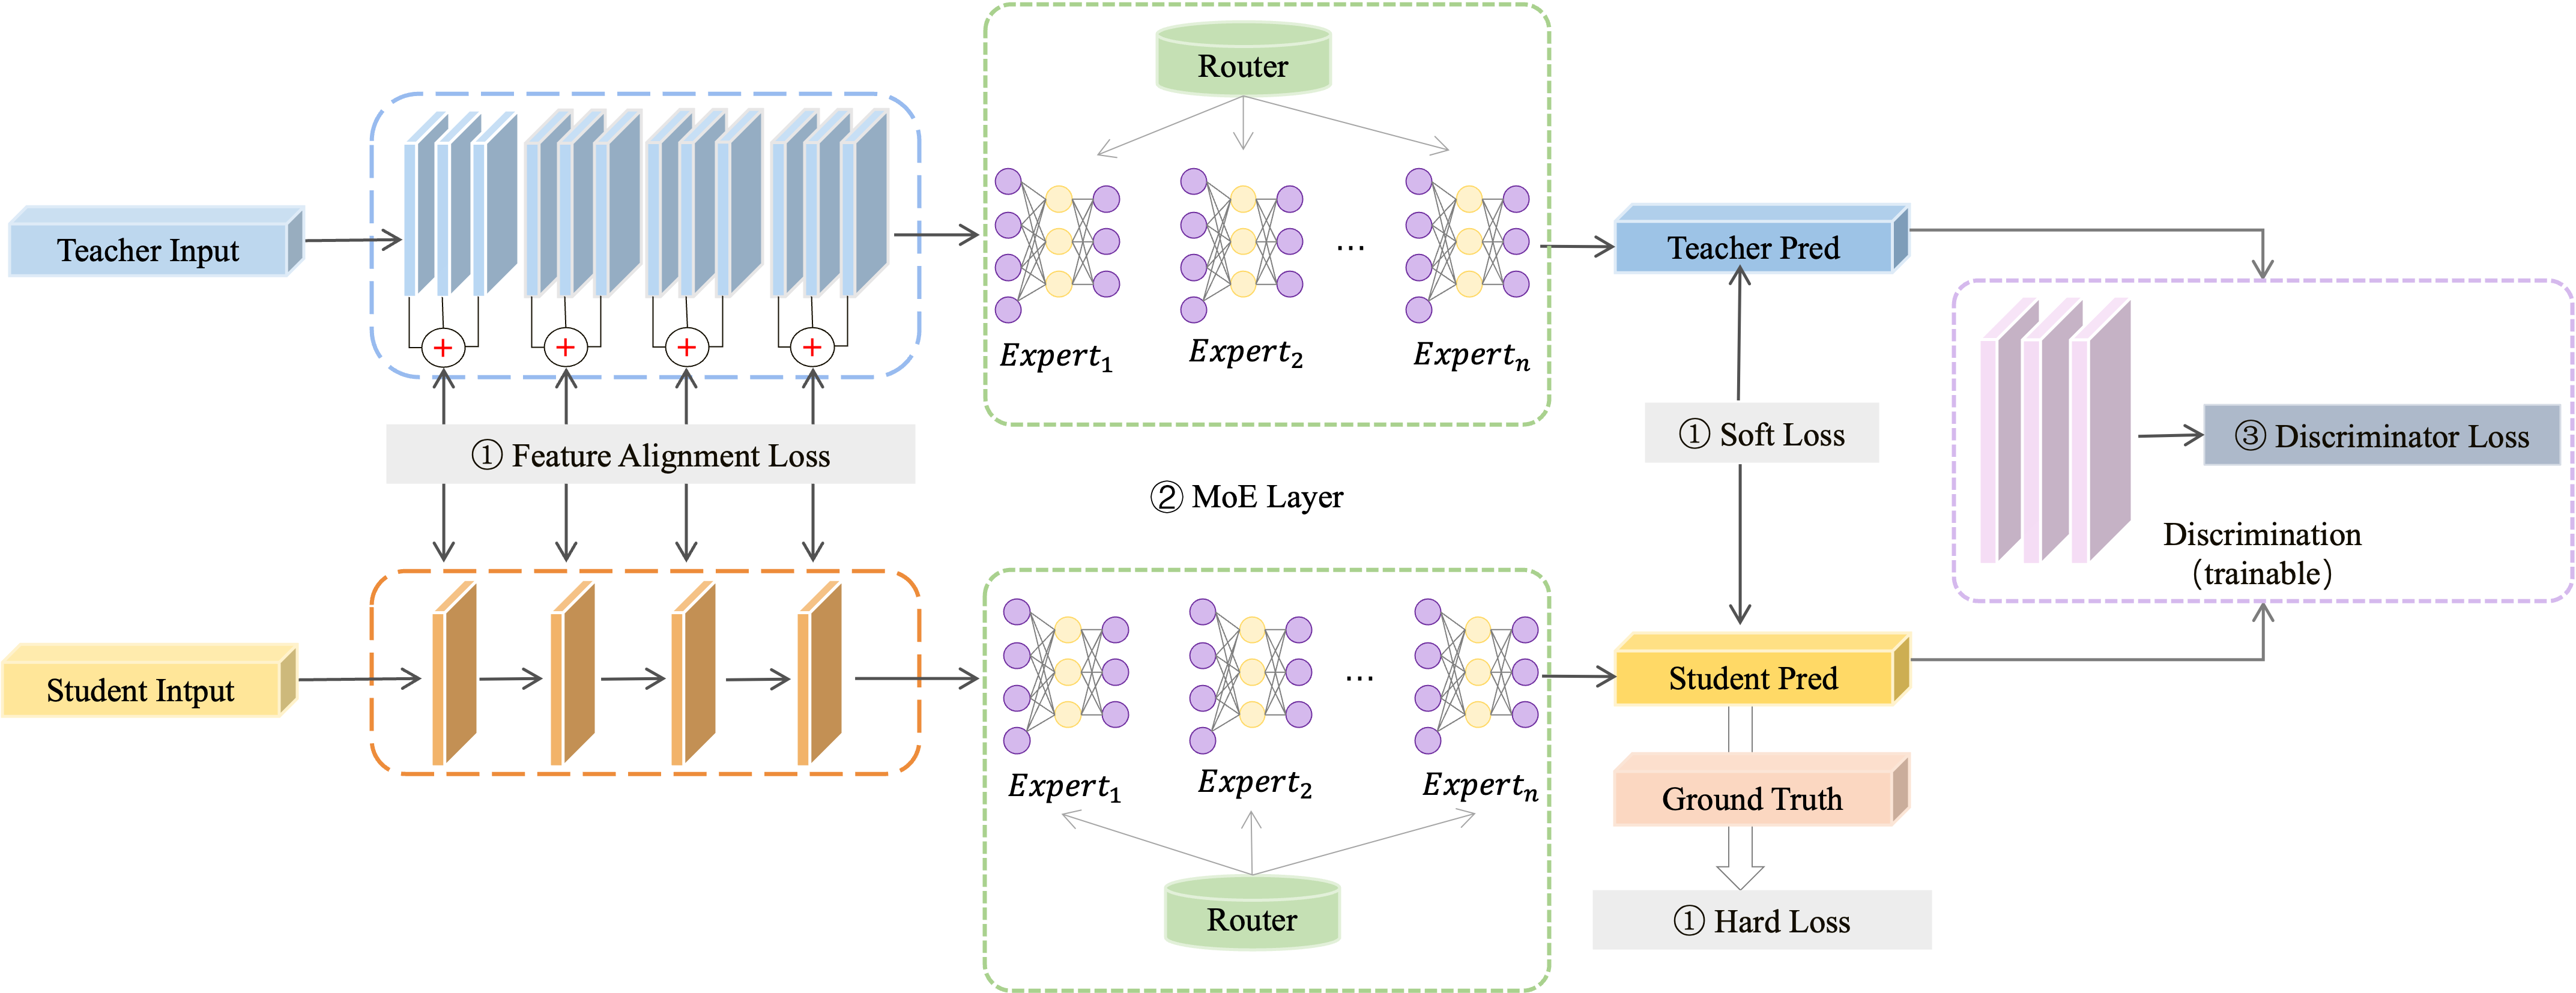
\includegraphics[width=\linewidth,height=0.84\textheight,keepaspectratio]{images/lrm+moe/micro-bert.png}

            {\usebeamerfont{caption}\usebeamercolor[fg]{caption}Source: \href{https://www.mdpi.com/2076-3417/14/14/6171}{Zheng et al. (2024)}}
        \end{figure}
    \framebreak
        \item \textbf{Other MoE Models}
        \begin{itemize}
            \item MoE variants of these families exist: the Switch Transformer is built on T5, and GLaM matches GPT-3 quality using an MoE architecture.
            \item MoE enables dynamic expert selection based on input.
            \item Improves learning efficiency and effectiveness.
        \end{itemize}
    \end{itemize}
\end{frame}